\documentclass[12]{article}
\usepackage[utf8]{inputenc}
\usepackage{float}
\usepackage{hyperref}
\usepackage{graphicx}
\date{\today}
\author{Carlos Bergillos, Roger Vilaseca, Adrià Cabeza}
\title{Creación de dietas para ancianos: \\ sistemas Basados en el conocimiento \\
	\large IA FIB @ UPC}
\usepackage[margin=1.25in]{geometry}
\usepackage{listings}
\lstset{
	    basicstyle=\ttfamily,
	    showstringspaces=false,
	    commentstyle=\color{orange},
	    keywordstyle=\color{blue},
	    breaklines=true,numbers=none,
	    stringstyle=\color{red}, tabsize=3,   
	    showstringspaces=false,
	    columns=flexible,
	}
\begin{document}
\maketitle
\vspace*{\fill}
\begin{center}

\includegraphics[scale=0.5]{images/UPClogo.png}
\end{center}
\newpage
\tableofcontents
\newpage
\section{Introducción} %CREC QUE DONE

Los \textbf{sistemas basados en el conocimiento (SBC)} son la parte de la Inteligencia Artificial donde se intenta hallar una solución utilizando el conocimiento. Hay ciertos problemas en la vida real que no se pueden resolver sin tener conocimiento específico sobre los elementos del dominio. 
\par
El motivo de esta práctica es comprender estos modelos de IA así que hemos atacado un problema con esta técnica: creación de menús para ancianos dependiendo de sus necesidades nutricionales y requisitos médicos. 
\par
Hemos desarrollado una ontología capaz de almacenar la información sobre los platos, los ingredientes, los nutrientes, las enfermedades y las limitaciones con \textbf{Protégé} y un sistema de reglas que describen el proceso de toma de decisiones usando \textbf{CLIPS}.
\par
Para atacar el problema de una manera adecuada hemos utilizado las diferentes fases de la metodología de ingeniería del conocimiento: 

\begin{itemize}
	\item \textbf{Identificación}, donde identificaremos el problema y sus características y requisitos. Además también concretaremos el dominio para poder identificar las fuentes de conocimiento necesarias para su desarrollo.%DONE
	\item \textbf{Conceptualización}, donde describiremos en profundidad los conceptos que intervienen en el dominio del problema y la descomposición de este último en subproblemas. %ALMOST DONE, FA FALTA AFEGIR INFO SOBRE ELS CONCEPTES QUE TENIM AL DOMINI
	\item \textbf{Formalización}, donde partiendo de los conceptos de la fase anterior, procediremos a su formalización desarrollando una ontología. También, para la resolución del problema formalizaremos el conocimiento y una metodología de resolución.
\item \textbf{Implementación}, donde dividiremos el problema en módulos para encapsular las diferentes partes del procedimiento en la resolución descrita en la fase anterior. Esta fase se basará en una metodología de desarrollo incremental, partiendo de un prototipo inicial que se va aumentando hasta conseguir un sistema final. 
\item \textbf{Prueba}, donde mediante juegos de prueba testearemos diferentes aspectos, en especial los más críticos, del sistema. 
\end{itemize}

\section{Identificación} %NOMÉS FALTA ESCRIURE AMB MÉS DETALL EL PROBLEMA
En este primer apartado del trabajo, describiremos el problema, sus distintas partes y fuentes de infromación que requieren. Además añadiremos un análisis de viabilidad de utilizar un SBC para su resolución.

\subsection{Descripción del problema}
% REESCRIURE I ALLARGAR, DEMANEN QUE SIGUI MÉS GRAN QUE EL PROPI ENUNCIAT
La alimentación es una pieza clave de nuestras vidas: nuestra manera de alimentarnos define nuestra salud. Con nuestra alimentación podemos prevenir el riesgo y agravamiento de enfermedades y mantener un nivel óptimo de salud. Es por eso que cuantos más años tenemos, más tenemos que vigilar nuestra alimentación.
\\
En esta práctica desarrollaremos una solución para este problema. Una solución basada en un sistema basado en el conocimiento que sea capaz de generar menús semanales personalizados adecuados a las características de una persona según su edad, sus restricciones de dieta considearndo sus enfermedades y sus preferencias generales sobre la comida. Por ejemplo, si una persona es vegetariana y además diabética se lo generaría un horari sin carne y con poca cantidad de azúcares. 

\subsection{Viabilidad de utilizar un SBC}
Si analizamos el problema podemos observar que no es un problema que se pueda resolver simplemente con algoritmos, sinó que el sistema requiere, para poder operar, de un conocimiento de nutrición salud.
\\
Además nuestro objetivo, como ya hemos mencionado anteriormente, es dada la información de un anciano como input es dar una solución viable. Así que un SBC parece una opción bastante apropiada para enfretarse al problema. 
\medskip

Pese a que se podría utilizar otros métodos como la satisfacción de restricciones o incluso mediante una búsqueda en el espacio de soluciones creemos que la mejor manera de aprovechar el conocimiento implícito que requiere el problema es usando la potencia que nos proporciona un sistema basado en conocmiento.

\subsection{Fuentes de conocimiento}

Nuestras fuentes de conocimiento se pueden dividir en dos grandes pilares:
\begin{itemize}
	\item \textbf{El usuario}: la persona que utilize nuestro sistema tendrá que indicar e introducir información acerca de su edad, sexo, enfermedades...para que podamos proporcionarle el mejor plan alimenticio. %maybe podem ser més específics amb el què preguntem i el perquè
	\item \textbf{Platos, ingredientes, enfermedades, nutrientes, etc}: el conjunto de conocimiento que necesita nuestro SBC para poder operar ha sido obtenido utilizando recursos en la red, especialmente se ha usado documentación especializada en el tema. 
\end{itemize}


\subsection{Objetivos y resultados esperados del sistema}
El objetivo final del problema es mostrar un menú para toda la semana que sea adecuado a las necesidades alimentícias del usuario. 
\medskip

Para esto el sistema tiene que cumplir una serie de objetivos: 
\begin{itemize}
	\item Obtener todos los datos del usuario que sean necesarios para poder utilizar el conocimiento del sistema y así poder devolver el mejor resultado posible
	\item Inferir sobre las características del usuario de forma que obtengamos un conjunto de platos específicos para el usuario
	\item Presentar al usuario el menú obtenido por el sistema		
\end{itemize}

Así pues esperamos de nuesto sistema un comportamiento que cumpla todos los objetivos indicados arriba para finalmente obtener unos resultados aceptables que esten concorde con el conocimiento del sistema. 
\section{Conceptualización}
En este apartado describiremos todos los conceptos del dominio. 

\subsection{Conceptos del dominio}
\begin{itemize}
\item \textbf{Persona}: las características necesarias para definir correctamente a la persona (usuario) son: \begin{itemize}
	\item \textbf{Edad}: tiene que ser $>=$ 65 ya que el sistema está orientado a ancianos
	\item \textbf{Género}: ya que dependiendo del sexo se tienen que seguir unas restricciones alimentícias u otras.
	\item \textbf{Nivel de ejercicio semanal}: que puede ser COMPLETAR
	\item \textbf{Enfermedades que padece}
	\item \textbf{Preferencias alimenticias}: que pueden ser Vegetariano, Vegano, COMPLETAR	
	\end{itemize}
	\item \textbf{Platos}
	\begin{itemize}
		\item \textbf{Temporadas}: pueden ser Otoño, Verano, Invierno y/o Primavera
		\item \textbf{Ingredientes}		
	\end{itemize}

	\item \textbf{Ingredientes}: las caracerístias necesarias para definir correctamente a un ingrediente son las siguientes: \begin{itemize}
		\item \textbf{Nutrientes} Los nutrientes que contiene el ingrediente en cuestión
		\item \textbf{Nombre}
		\item \textbf{Temporadas}: pueden ser Otoño, Verano, Invierno y/o Primavera
		\item \textbf{Tipo}: \begin{itemize}
			\item \textbf{FICAR}
			\item \textbf{ELS}
			\item \textbf{DIFERENTS TIPUS D'INGREDIENTS QUE TENIM}
			\end{itemize}
		\end{itemize}
	\item \textbf{Nutrientes}: formado por los valores nutricionales que hemos considerado más importantes y adecuados para realizar nuestro sistema. Entre ellos se encuentran: 
	\begin{itemize} 
		\item \textbf{Grasa}
		\item \textbf{Carbohidratos}
		\item \textbf{Calorías}
		\item \textbf{Sucrosa}
		\item \textbf{Glucosa}
		\item \textbf{Fructosa}
		\item \textbf{Lactosa}
		\item \textbf{Cafeína}
		\item \textbf{Alcohol}
		\item \textbf{Azúcar}
		\item \textbf{Colesterol}
		\item \textbf{Grasas de las cuáles saturadas}
		\item \textbf{Vitamina B5}
		\item \textbf{Vitamina B6}
		\item \textbf{Vitamina B12}
	\end{itemize}


\item \textbf{Enfermedades}: cada enfermedad, además de su nombre la cual nos sirve para definirla en sí, tenemos para cada enfermedad el conocimiento de qué limitaciones alimentícias presentan. \begin{itemize}
	\item \textbf{Nombre}
	\item \textbf{Limitaciones}: pueden ser limitaciones asociadas a nutrientes o a ingredientes.
\end{itemize}




\end{itemize}

\subsection{Problemas y subproblemas}

Uno de los mejores métodos para trabajar con grandes problemas como este es dividirlos en varios subproblemas más pequeños para poderlo solucionar.

En nuestro caso lo vamos a dividir entre los siguientes 4:

\subsubsection{Recogida de información personal}

En esta parte del problema realizaremos varias preguntas al usuario (descritas en el apartado anterior), donde obtendremos la suficiente información para luego poder ser usado y obtener un menú adecuado a las condiciones y gustos de la persona.

\subsubsection{Análisis de los datos personales}

Una vez obtenidos los datos de la persona, el experto clasificará mediante una puntuación los diferentes platos según lo adecuados que sean para la persona. En esta parte también vamos a descartar aquellos platos que la persona no pueda tener en su menú en ninguna circunstancia.

\subsubsection{Filtrado de platos para el menú}

Vamos a coger los diferentes platos y los vamos a repartir mediante ... FALTA ACABAR UN COP DECIDIM L?ALGORITME FINAL

\subsubsection{Impresión del menú}

Una vez tengamos el menú construido vamos a sacar por pantalla el menú final de la semana, donde por cada plato habrá sus ingredientes.
Después del menú va a salir la información nutricional del menú obtenido, comparados con los resultados que deberíamos tener a partir de la información que nos ha dado la persona en el primer subproblema.

\subsection{Ejemplos del conocimiento extraído del dominio}
%aquí deberíamos explicar como hemos ido desarrollando prototipos de la implementación para demostrar que hemos usado una metodología incremental 
A partir de información que obtenemos del dominio podemos llegar a clasificar los platos en función de las características y peticiones de cada persona.

Por ejemplo a partir de las siguientes características o preferencias que podríamos obtener a partir de las preguntas hechas, obtendríamos los siguientes resultados.

\begin{itemize}
	\item En el caso de los vegetarianos vamos a quitar de los posibles platos aquellos que tengan algún ingrediente del tipos carne.
	\item Si la persona tuviera diabetes vamos a intentar que los platos sugeridos tengan poca cantidades de azúcares.
	\item En cambio si la persona responde que le gusta un alimento en concreto vamos a puntuar de una forma más alta aquellos platos que contengan el alimento en cuestión.
\end{itemize}

\subsection{Flujo de razonamiento}

Para poder clasificar correctamente los platos en nuestro problema a partir de las preguntas hechas.

Primero de todo pasaremos un filtro donde se eliminaran del conjunto de platos, aquellos que la persona no puede tomar en ninguna circunstancia.

A continuación los platos que hayan pasado de la opción anterior serán puntuados para prioriza que platos debe o no debe tomar dicha persona.

Al final obtendremos una lista ordenada de los mejores platos para la persona, con los cuales diseñaremos el menú más adecuado para cada usuario. 


\section{Formalización}

\subsection{Desarrollo de la ontología}
Para desarrollar correctamente la ontología hemos procurado que todos los conceptos del dominio sean representables. En este caso, los términos más importantes de la ontología son los \textbf{platos}, puesto que nuestra solución será un conjunto de ellos, los \textbf{ingredientes} y sus \textbf{características nutricionales} y los conceptos relacionados con el usuario: \textbf{preferencias} y \textbf{enfermedades}. Además para poder representar bien los susodichos conceptos, hemos creído conveniente hacer uso de clases auxiliares para definir cantidades. Así pues, por ejemplo para definir que un plato contiene una cantidad de un ingrediente en concreto usaríamos la clase \textit{IngredientQuantity}.
\label{ontologia_apartado}
\subsubsection{Definición de clases y jerarquía}

La ontología que hemos realizado para nuestro SBC contiene diversas clases. Se puede observar en la figura %\ref{ontologia}

\begin{figure}[H]
\centering
\includegraphics{images\fulllight.png}
\caption{Ontología de nuestro SBC}
\label{ontologia}
\end{figure}


\textbf{class\_menu}
\begin{figure}[H]
\centering
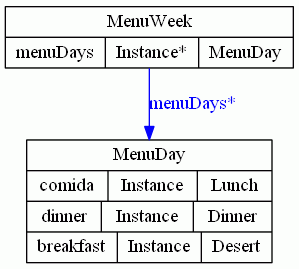
\includegraphics[scale=0.5]{images/classMenu.png}
\caption{Clase Menu}
\label{menu}
\end{figure}

Definimos toda la información de un menú en esta clase. Tenemos la cantidad de días que contiene nuestro plan alimenticio y disitintas instancias de menús diarios los cuales contienen información acerca de sus comidas mediante a sus instancias desayuno, comida y cena. 
\\

Los atributos son: 
\begin{itemize}
\item \textbf{menuDays}: menú diario
	\begin{itemize}
	\item comida: comida de un menú diario
	\item dinner: cena de un menú diario
	\item breakfast: desayuno de un menú diario
	\end{itemize}
\end{itemize}

\vspace{0.5cm}

\textbf{class\_Course}
\begin{figure}[H]
\centering
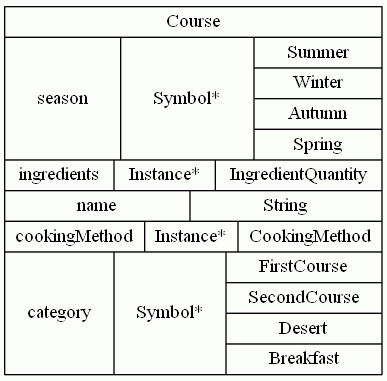
\includegraphics[scale=0.5]{images/classCourse.png}
\caption{Clase Platos}
\label{platos}
\end{figure}

Definimos aquí toda la información que contiene un plato. Tenemos información acerca de qué estación pertenece el plato, los ingredientes que contiene y sus cantidades además de la categoría a la que pertenece que puede ser primer plato, segundo plato, postre o desayuno, 
\\

Los atributos son:
\begin{itemize}
\item \textbf{season}: estación del año; puede ser Otoño, Verano, Invierno o Primavera
\item \textbf{ingredientes}: ingredientes que contiene un plato y su cantidad
\item \textbf{name}: nombre del plato
\item \textbf{category}: categoría del plato; puede ser primer plato, segundo plato, desayuno o postres. 
\end{itemize}


\vspace{0.5cm}

\textbf{class\_Ingredient}
\begin{figure}[H]
\centering
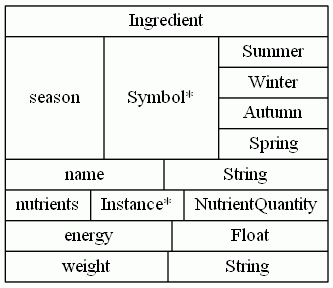
\includegraphics[scale=0.5]{images/classIngredient.png}
\caption{Clase Ingredientes}
\label{ingredientes}
\end{figure}

Definimos aquí toda la información que contiene un ingrediente. Tenemos de manera parecida a los platos, una estación asociada al ingrediente. Por ejemplo: las castañas estarían asociadas al otoño. Además también disponemos de los valores nutricionales que presenta el ingrediente.
\\

Los atributos son: 

\begin{itemize}
\item \textbf{season}: estación del año; puede ser Otoño, Verano, Invierno o Primavera
\item \textbf{name}: nombre del ingrediente
\item \textbf{nutrients}: nutrientes del ingrediente
\end{itemize}


\vspace{0.5cm}

\textbf{class\_IngredientQuantity}
\begin{figure}[H]
\centering
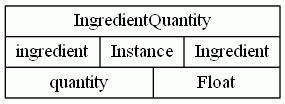
\includegraphics[scale=0.5]{images/classIngredientQuantity.png}
\caption{Clase Enfermedad}
\label{cantidad_ingrediente}
\end{figure}

Para poder expresar la cantidad de ingredientes que contiene un plato hacemos uso de esta clase la cual contiene una referencia a una instancia ingrediente y la cantidad que hay en ese plato del ingrediente.
\\

Los atributos son: 
\begin{itemize}
\item \textbf{ingredient}: ingrediente
\item \textbf{quantity}: cantidad del ingrediente
\end{itemize}


\vspace{0.5cm}

%\textbf{class\_Nutrients}
%\begin{figure}[H]
%\centering
%\includegraphics[scale=0.5]{images/classNutrient.png}
%\caption{Clase Nutrientes}
%\label{nutrientes}
%\end{figure}

Definimos en esta clase toda la información que contiene un nutriente... TODO FINISH IT 
\\
TODO continuar amb els atributs
%Los atributos son:
%\begin{itemize}
%\item \textbf{}
%\item \textbf{}
%\end{itemize}


\vspace{0.5cm}

\textbf{class\_NutrientQuantity}
\begin{figure}[H]
\centering
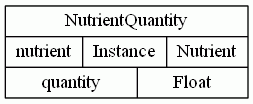
\includegraphics[scale=0.5]{images/classNutrientQuantity.png}
\caption{Clase Cantidad de Nutrientes}
\label{cantidad_nutriente}
\end{figure}

Para poder expresar la cantidad de nutrientes que contiene un ingrediente en concreto hacemos uso de esta clase. Esta dispone de una referencia a una instancia de nutriente además de la cantidad que ese nutriente en ese ingrediente (las unidades han sido normalizadas en gramos). 
\\

Los atributos son: 
\begin{itemize}
\item \textbf{nutrient}: nutriente
\item \textbf{quantity}: cantidad del nutriente
\end{itemize}


\vspace{0.5cm}

\textbf{class\_Disease}
\begin{figure}[H]
\centering
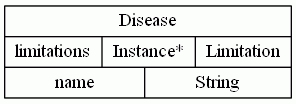
\includegraphics[scale=0.5]{images/classDisease.png}
\caption{Clase Enfermedad}
\label{enfermedad}
\end{figure}

Definimos en esta clase toda la información que contiene una enfermedad. En nuestro caso, una enfermedad presenta una serie de limitaciones alimentícias que pueden estar referidas a un ingrediente o a un tipo de nutriente. 
\\

Los atributos son: 
\begin{itemize}
\item \textbf{limitations}: limitaciones alimentícias que suponen la enfermedad
\item \textbf{name}: nombre de la enfermedad
\end{itemize}

\vspace{0.5cm}

\textbf{class\_Limitation}
\begin{figure}[H]
\centering
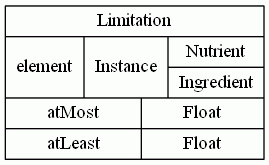
\includegraphics[scale=0.5]{images/classLimitation.png}
\caption{Clase Limitación}
\label{limitacion}
\end{figure}

Para ser capaces de expresar una limitación o incluso una preferencia alimentícia, hemos hecho uso de esta clase para poder relacionar un nutriente o un ingrediente con una limitación de cantidad AtMost(como máximo) o atLeast(como mínimo).
\\

Los atributos son:
\begin{itemize}
\item \textbf{element}: elemento sobre el que se aplica la limitación, puede ser un nutriente o un ingrediente
\item \textbf{atMost}: valor que representa el tope máximo necesario para cumplir la limitación
\item \textbf{atLeast}: valor que representa el mínimo necesario para cumplir la limitación
\end{itemize}



%explicar detalladamente como se ha construido la ontología

\subsection{Método de resolución}

 explicar problemas que intervienen en la resolución
% Descripción del proceso de resolución y como se organizasn los problemas y subproblemas
\section{Implementación}

\subsection{Creación de la ontología}
%TODO: REPASSAR, DEMANAR A EN CARLOS COM HO VEU
Para generar la ontología hemos usado el programa Protégé añadiendo las diferentes características anteriormente mencionadas en los apartados% \ref{ontologia_apartado}
\\
En cuanto a las instancias, hay una distinción básica entre ellas: estáticas y dinámicas. Hay algunas que se han creado dinámicamente durante la ejecucción del programa como podrían ser Persona o MenúDía. Para las estáticas en cambio (Nutriente, Plato, Ingrediente, IngredienteCantidad, NutrienteCantidad, Enfermedad o Limitaciones) hemos usado diversas bases de datos y un script en python para crearlas a priori y tener los archivos .pins necesarios. 
\subsection{Módulos}
\\
\\
THIS GOTTA BE WRITTEN STILL\\
\\
\\
\subsection{Prototipos}
%ES POT ALLARGAR I MILLORAR, FET PQ HO POSA A LES RÚBRIQUES
Tal y como se ha mencionado anteriormente, hemos seguido para el desarrollo de la práctica un método incremental por prototipos. Este tipo de desarrollo nos ha permitido avanzar de manera más organizada y paulatina. 
\\
En un inicio, desarrollemos nuestro \textbf{prototipo inicial}: una ontología bastante completa (muy parecida a la que se ha utilizado en la versión final) y un sistema que hacía preguntas y creaba un menú totalmente random.  Nos sirvió para empezar a familiarizarnos con \textbf{Protégé} y \textbf{CLIPS} y en cómo tenían que ser las instancias. Después iteremos sobre ese prototipo: creemos un script en \textbf{Python} para facilitarnos la creación de las instancias y empezemos a añadir las primeras reglas básicas (i.e. restricciones de vegetariano). 
\\
Entonces después de hacer unos pequeños cambios en la ontología y por consiguiente en el script para crear instancias, procedimos a crear, de manera progresiva, las diferentes reglas inherentes al conocimiento.  

\section{Juego de Prueba}
%fer-ne més de 6 (lo que consideren un bon número)
Una vez implementado nuestro SBC, hemos realizado una serie de pruebas enfocadas a testear diferentes puntos de la aplicación. Así pues, mediante estas pruebas, hemos podido comprovar el correcto funcionamento del sistema, tanto a nivel general como a nivel particular.

\subsection{Prueba 1: }
\subsection{Prueba 2: }
\subsection{Prueba 3: }
\subsection{Prueba 4: }
\subsection{Prueba 5: }
\subsection{Prueba 6: }
\section{Conclusión}
Podemos concluir que hemos aprendido sobre SBC y sobre el desarrollo de éstos pues hemos sido capaces de desarrollar un SBC functional basado en otologías y reglas de producción.
\medksip

No obstante, cabe mencionar que debido a la complejidad inherente a la representación del conocimiento y el poco tiempo del que se ha dispuesto para realizar la práctica, el sistema podría ser mejorado con más conocimiento y más instancias. 
\\

A pesar de eso, hemos profundizado en el subcampo de los SBC y hemos conseguido realizar uno con utilidad práctica, que cumple los objetivos y resultados esperados.

\end{document}

